%!TEX root = ../main.tex

\chapter{Double-beta decay}\label{chap:theory}

Studying the properties and interactions of neutrinos has been one of the most
exciting and vigorous activities in particle physics and astrophysics ever
since W.~E.~Pauli in 1930~\cite{Brown1978}. Despite their weakly interacting
nature, that challenged physicists to detect it directly until
1965~\cite{Cowan1956}, we have so far accumulated an enormous amount of
knowledge about them. No experiments that have been performed so far have
detected conclusive deviations from the Standard Model, except neutrino
oscillation experiments, which have shown that neutrinos are massive and
mixed~\cite{Fukuda1998, Ahmad2002, Eguchi2003, Kajita2016, McDonald2016}.
This discovery, however, is far from being the last word on neutrino
fundamental properties. The mechanism through which the neutrino acquires mass
and why it is so tiny with respect to all the other elementary
particles remains a mystery. How can such a specific and rare nuclear process
like double-beta decay help shading some light on these enigmas?

The mass-generation mechanism is strongly connected to the nature of these
particles, which could be either of Dirac or Majorana type (i.e.~neutrino and
anti-neutrino are distinct particles or the same particle). An attempt to
address this problem is done by experiments looking for the neutrinoless mode
of double-beta decay. The double-beta decay, in its two-neutrino Standard Model
mode (\nnbb), consists in a nucleus that decays into a daughter nucleus with
two electrons and two electron anti-neutrinos as a byproduct. If the neutrino
is a Majorana particle then another mode may occur (\onbb), in which
neutrinos are not produced at all~\cite{Schechter1982}. Neutrinoless
double-beta decay experiments are considered the most promising way to solve
the neutrino mass puzzle, although these events are very rare processes
controlled by weak interactions.

From its definition it is also clear that neutrinoless double-beta decay
violates lepton number conservation, an accidental symmetry in the Standard
Model, by two units ($\Delta L = 2$). The existence of such a process beyond
the Standard Model would therefore be crucial to support baryogenesis ideas,
that try to explain why we live in matter-dominated Universe.

In the following the theory of double-beta decay is briefly reviewed, focusing
on the core concepts and formulas which will be used in this work. Formulas for
the differential double-beta decay rates associated to the two-neutrino mode,
the neutrinoless mode as well as modes driven by other new physics scenarios
(Majoron emission, Lorentz symmetry violation) are given. \fillme{fillme}

\section{Two-neutrino double-beta decay}\label{sec:nbb:2nbb}

The two-neutrino double-beta decay (\nnbb) processes, first suggested by
M.~Goeppert-Mayer in 1935~\cite{GoeppertMayer1935}, can be schematically
represented as:
\[
  \begin{array}{llr}
    2\nu\beta^-\beta^-: &
      \mathcal{N}(A,Z) \longrightarrow \mathcal{N}(A,Z+2)+2e^-+2{\overline \nu}_e & \\
    2\nu\beta^+\beta^+: &
      \mathcal{N}(A,Z) \longrightarrow \mathcal{N}(A,Z-2)+2e^++2\nu_e &,
  \end{array}
\]
where \NAZ\ represents a nucleus with mass number $A$ and atomic number $Z$. The
\nnbbm\ (\nnbbp) process consists of the simultaneous $\beta^-$ ($\beta^+$)
decay of two neutrons (protons) in the same nucleus. The processes are
generated at second-order in the perturbative expansion of weak interactions in
the Standard Model. The Feynman graph for \nnbbm\ is shown in
\cref{fig:nbb:feydiag}, left.

\begin{figure}
  \centering%
  \makebox[\textwidth]{%
    \includegraphics[width=0.5\textwidth]{plots/theory/2nbbfey.pdf}%
    \includegraphics[width=0.5\textwidth]{plots/theory/0nbbfey.pdf}%
  }
  \caption{%
    Feynman graphs for two-neutrino (left) and neutrinoless (right) double-beta
    decay.
  }\label{fig:nbb:feydiag}
\end{figure}

Since the \nnbb\ decays have a four-body leptonic final state, the sum of the
kinetic energies of the two decay electrons follows a continuous distribution
from zero to the Q-value of the decay process (the recoil energy of the final
nucleus is negligible), which is given by
\[
  Q_{\beta\beta} = M_i - M_f - 2m_e \;,
\]
where $M_i$ and $M_f$ are, respectively, the masses of the initial and final
nuclei (i.e.~the energy levels of their ground states; if the transition occurs
into an excited energy level of the final nucleus, $M_f$ must be replaced with
the appropriate energy).

A nucleus \NAZ\ can decay through a \nnbb\ process if its ground state has an
energy which is larger than the ground-state energy of the nucleus
$\mathcal{N}(A,Z\pm2)$ plus twice the electron mass. Moreover, if a nucleus can
decay through both the \b\ and \nnbb\ processes, in practice the latter is not
observable, because its \b\ decay lifetime is much shorter than its \nnbb\
decay lifetime (the half-life of \nnbb\ is typically around $10^{19}-10^{24}$
yrs). Therefore, in practice the \nnbb\ decay of a nucleus is observable only
if its \b\ decay is energetically forbidden or strongly suppressed because of a
large change of spin. The $\beta^-$ decay of a nucleus \NAZ\ is energetically
forbidden if its ground-state energy is lower than the ground-state energy of
the nucleus $\mathcal{N}(A,Z+1)$ plus the electron mass ($Q_{\beta^{-}} < 0$).
Typically, in \nnbbm\ decays the energy levels of the three nuclei \NAZ,
$\mathcal{N}(A,Z+1)$, and $\mathcal{N}(A,Z+2)$ are of the type depicted in
\cref{fig:nbb:gesixlevels}, left, where the specific case of \gesix,
$^{76}$As, and $^{76}$Se nuclei is considered.

\begin{figure}
  \centering
  \makebox[\textwidth]{%
    \includegraphics[width=0.5\textwidth]{plots/theory/gesix-levels.pdf}%
    \includegraphics[width=0.5\textwidth]{plots/theory/masspar.pdf}%
  }%
  \caption{%
    On the left: schematic illustration of the energy level structure of the
    $2\nu\beta^-\beta^-$ decay of \gesix into $^{76}$Se. On the right: general
    energy level configuration for double-beta decay emitters.  The situation
    for a nucleus with even mass number $A$ is presented: the mass parabola,
    representing the dependence of the binding energy $M(A,Z)$ on the atomic
    number $Z$, is plotted for even-even (even number of protons and neutrons)
    and odd-odd nuclei with the relevant \b\ and \b\b\ decays among them.
  }\label{fig:nbb:gesixlevels}
\end{figure}

\marginnote{$2\nu\beta^-\beta^-$}
The naturally occurring isotopes which can decay through the
$2\nu\beta^-\beta^-$ process, with forbidden or suppressed $\beta^-$ decay are
35, and they are listed in~\cite{Giunti2007}. All of the initial and final
nuclei in the \nnbbm\ process are even-even, i.e.~they have an
even number of protons and neutrons. Their binding energy is larger than the
intermediate odd-odd nuclei one because of the pairing force acting between
identical nucleons (see \cref{fig:nbb:gesixlevels}, right). For the same reason,
all of the initial and final nuclei have a $0^+$ ground state.  Therefore, all
ground-state to ground-state transitions are $0^+\rightarrow0^+$. Ground-state
transitions to an excited state of the final nucleus may be energetically
allowed, as in the case of the $^{76}\text{Ge} \rightarrow {^{76}\text{Se}}$ decay in
\cref{fig:nbb:gesixlevels}, left, in which there is an accessible $2^+$ excited
state of $^{76}$Se. However, due to a cancellation occurring in the phase
space integral and the lower Q-value~\cite{Tomoda1991}, the
$0^+\rightarrow2^+$ double-beta decay is suppressed with respect to
$0^+\rightarrow0^+$.

\marginnote{$2\nu\beta^+\beta^+$}
There are only six naturally occurring isotopes which can decay through the
\nnbbp\ process~\cite{Haxton1985}. These isotopes have small Q-values and
lifetimes which are much longer than the lifetimes of the \nnbbm. The reason
for the rarity of \nnbbp-decaying isotopes and their small Q-values can be
understood considering that the decay $\mathcal{N}(A,Z) \rightarrow
\mathcal{N}(A,Z-1)$ can occur in two ways:
\[
  \begin{array}{lrl}
    \beta^+: &
      \mathcal{N}(A,Z) \rightarrow \mathcal{N}(A,Z-1) + e^+ + \nu_e & \\
    \text{EC}: &
      e^- + \mathcal{N}(A,Z) \rightarrow \mathcal{N}(A,Z-1) + \nu_e &.
  \end{array}
\]
Since $Q_\text{EC} = Q_{\beta^+}+2m_e$, the electron-capture process (EC) can
occur even if the $\beta^+$ process is energetically forbidden ($Q_{\beta^+} <
0$). Thus, in order to have an energetically forbidden
$\mathcal{N}(A,Z)\rightarrow\mathcal{N}(A,Z-1)$ transitions, the ground-state
energy of \NAZ\ must be smaller than the ground-state energy of the nucleus
$\mathcal{N}(A,Z-1)$ minus the electron mass ($Q_\text{EC}<0$).  Considering as
a reference the energy of the ground-state energy of the intermediate nucleus,
the ground-state energy of the initial nucleus in a \nnbbp\ decay must be at
least $2m_e$ lower than in the case of a \nnbbm\ decay. This implies that
\nnbbp-decaying isotopes are more rare than \nnbbm-decaying isotopes. Moreover,
for the same energy difference between the ground states of the intermediate
and final nuclei, the energy difference between the ground states of the
initial and final nucleus in a \nnbbp\ decay is at least $2m_e$ lower than in
the case of a \nnbbm\ decay, leading to a correspondingly smaller Q-value. For
these reasons, the \nnbbp\ decay has been less studied than the \nnbbm\ decay
and in the following we will consider only \nnbbm\ decays (from now on we will
simply refer to them with \nnbb). Let us only mention that $\mathcal{N}(A,Z)
\rightarrow \mathcal{N}(A,Z-2)$ transitions can occur not only through \nnbbp\
processes, but also through the processes \fillme{fillme}
\[
  \begin{array}{lrl}
    \text{EC}\beta^+: &
      e^- + \mathcal{N}(A,Z) \rightarrow \mathcal{N}(A,Z-2) + e^+ + 2\nu_e & \\
    2\text{EC}2\nu: &
      2e^- + \mathcal{N}(A,Z) \rightarrow \mathcal{N}(A,Z-2) + 2\nu_e &.
  \end{array}
\]

\marginnote{decay \\ rate}
The rate of \nnbb\ can be calculated by invoking the recipe of the Fermi golden
rule for simple $\beta$ decay. To a good approximation, the decay width can be
factorized as a kinematic part (the phase space of the leptons emitted in the
decay) times a nuclear part (the matrix element responsible for the transition
probability between two nuclear states):
\[
  \Gamma^{2\nu} = G^{2\nu}(Q_{\beta\beta},Z) |\mathcal{M}^{2\nu}|^2 \;,
\]
where $G^{2\nu}$ is obtained by integration over the phase space of four
leptons emitted in the decay and can be calculated exactly. The nuclear matrix
element $\mathcal{M}^{2\nu}$ deals with the nuclear structure of the transition
and is much more difficult to evaluate.

Denoting the 4-momentum of the two electrons and the two anti-neutrinos by
$p^\alpha_i=(E_i,\mathbf{p}_i)$ and $q^\alpha_i=(\omega_i,\mathbf{q}_i)$,
respectively ($i=1,2$), the relevant matrix element is given by
\[
  i\mathcal{M} = iG^2_F V^2_{ud} [\bar{u}(p_1) \gamma^\mu (1-\gamma_5) v(q_1)]
                 [\bar{u}(p_2) \gamma^\nu (1-\gamma_5) v(q_2)] J_{\mu\nu} -
                 (p_1\leftrightarrow p_2) \;.
               \]
(the last expression in brackets represents the first term with $p_1$ and $p_2$
interchanged).  The hadronic tensor $J_{\mu\nu}$ corresponds to the product of
two nuclear currents written in the impulse approximation~\cite{Tomoda1991}.
Including the implementation of the long-wave and closure approximation for the
hadronic tensor~\cite{Tomoda1991}, we obtain
\[
  \sum_\text{spin} |\mathcal{M}|^2 = 64 G^4_F |V_{ud}|^4 g^4_A (p_1 \cdot p_2)
                                     (q_1 \cdot q_2) |\mathcal{M}^{2\nu}|^2 \;,
\]
where the nuclear matrix element involves vector and axial couplings for Fermi
and Gamow-Teller transitions in the form
\[
  g^2_A\mathcal{M}^{2\nu} = g^2_V \mathcal{M}^{2\nu}_F -
                            g^2_A \mathcal{M}^{2\nu}_{GT} \;.
\]

General methods for phase-space factor calculations in double-beta decay have
been developed~\cite{Doi1981,Doi1983,Tomoda1991}. The decay rate is given by
integrating over all possible energies and angles of the leptons emitted in the
decay. For the two-neutrino mode, these leptons are the two electrons and the
two anti-neutrinos:
\[
  \begin{split}
    %G^{2\nu} \propto \int \text{d}^3p_1\text{d}^3p_2\text{d}^3q_1\text{d}^3q_2F(Z,E_1)F(Z,E_2)\delta(E_1+E_1+\omega_1+\omega_2-E_F+E_I)\;,
    \text{d}\Gamma = \frac{1}{4} \int & \frac{\text{d}^3p_1}{(2\pi)^32E_1}
                                        \frac{\text{d}^3p_2}{(2\pi)^32E_2}
                                        \frac{\text{d}^3q_1}{(2\pi)^32\omega_1}
                                        \frac{\text{d}^3q_2}{(2\pi)^32\omega_2} \\
                                      & \times F(Z,E_1) F(Z,E_2) \sum |\mathcal{M}|^2 \\
                                      & \times 2\pi\delta (E_1 + E_2 + \omega_1 +
                                        \omega_2 - E_F + E_I) \;, \\
  \end{split}
\]
where $F(Z,E)$ is the Fermi function that describes the Coulomb effect on the
outgoing electrons and $E_I$, $E_F$ are the energies of the parent and the
daughter nucleus, respectively.

In the Primakoff–Rosen approximation~\cite{Primakoff1959} for the
non-relativistic Coulomb correction, the sum spectrum of the electrons energies
can be analytically calculated. After a suitable change of integration
variables and defining the sum of kinetic energies $K=T_1+T_2$ for the two
electrons and integrating over the remaining variables, we obtain
\begin{equation}\label{eq:nbb:stdmodel}
  \frac{\text{d}\Gamma}{\text{d}K} = \Lambda \cdot (K^5+10K^4+40K^3+60K^2+30K)
                                     (Q_{\beta\beta}-K)^5 \;,
\end{equation}
where $K$ is written in units of the electron mass. The overall constant factor
is given by
\[
  \Lambda = \frac{G_F^4g_A^4|V_{ud}|^4F^2_\text{PR}(Z)m_e^{11}}{7200\pi^7}
            |\mathcal{M}^{2\nu}|^2 \;,
\]
with $F_\text{PR}(Z) = 2\pi\alpha/Z(\-e^{-2\pi\alpha Z})$. The distribution for
\gesix\ is plotted in \cref{fig:nbb:spectra}.

\begin{figure}
  \centering
  \includegraphics{plots/theory/bb-spectra.pdf}
  \caption{%
    Two-electron energy spectra for the two-neutrino and the neutrinoless
    double-beta decay modes of \gesix. Analytic formulas, obtained with the
    Primakoff-Rosen approximation for the Fermi function, are taken
    from~\cite{Tretyak1995, Tretyak2002}.
  }\label{fig:nbb:spectra}
\end{figure}

\section{Neutrinoless double-beta decay}\label{sec:nbb:0nbb}

The neutrinoless double-beta decay processes (\onbb) of the types
\[
  \begin{array}{lrl}
    0\nu\beta^-\beta^-: &
      \mathcal{N}(A,Z) \longrightarrow \mathcal{N}(A,Z+2)+2e^- & \\
    0\nu\beta^+\beta^+: &
      \mathcal{N}(A,Z) \longrightarrow \mathcal{N}(A,Z-2)+2e^+ &,
  \end{array}
\]
which have been proposed by W.~H.~Furry in 1939~\cite{Furry1939}, are forbidden
in the minimal Standard Model, where the neutrinos are massless, because the
conservation of the total lepton number is violated by two units.
Interestingly, lepton number $L$ (as well as baryon number $B$) is only an
accidentally conserved global symmetry in the Standard Model and its
conservation in extended theories seems very unlikely. To support the idea that
$L$ and $B$ conservation laws are nothing sacred and lack of a deep
justification even in the Standard Model, one should note that they are only
valid at the classical level\footnote{Chiral anomalies actually violate this
conservation law. It can be shown that the currents associated with baryon
and lepton number have non-vanishing divergences: $\partial^\mu J_\mu^{B,L} =
c G_{\mu\nu} \widetilde{G}^{\mu\nu} \neq 0$, where $G_{\mu\nu}$ is the
electroweak gauge field strength and $J_\mu^B = \sum \overline{q}_i \gamma_\mu
q_i$, $J_\mu^L = \sum \overline{l}_i \gamma_\mu l_i$.}. In the effective field
theory framework, one can easily realize that the (unique) lowest higher dimensional
$d=5$ operator one can write down,
\[
  \mathcal{L}_\text{eff} = \frac{1}{2} \frac{h_{\alpha\beta}}{\Lambda}
                           (\overline{L_\alpha^c}\widetilde{\Phi})
                           (\widetilde{\Phi}^T L_\beta) + \text{h.c.} \;,
\]
often referred to as Weinberg operator~\cite{Weinberg1979}, immediately
violates lepton number. Superscript $^c$ denotes the charge conjugation
operation, $L_\alpha = (\nu_\alpha, \alpha)^T$ are the lepton doublets of
flavor $\alpha = e, \mu, \tau$, $\Phi$ is the Higgs doublet and $\Lambda$
denotes the energy scale of the complete theory. Therefore, it
is possible to suspect that the validity of $B$ and $L$ conservation laws is
just approximate or circumstantial, since it is related to the range of
energies that we can explore in laboratories.

Why searching for lepton violation is so important? Apart from the naturalness
issue, the connection with baryon number in most Grand Unified Theories (GUTs),
i.e.~gauge theories with a single gauge coupling at a certain high energy
scale, might help solving the long-standing problem of explaining why we live
in a matter-dominated Universe, often referred as the `baryogenesis problem',
despite the equal importance of matter and anti-matter in the Standard Model.
In 1967, Sakharov proposed a set of necessary conditions to generate the cosmic
baryon asymmetry~\cite{Sakharov1991}. These conditions are satisfied in the
Standard Model, but they don't generate the required amount of baryonic
asymmetry observed by current experiments~\cite{citation needed}. One viable
and attractive way to mach theoretical predictions to experimental data is
assuming that lepton number violating processes had a major role in the early
history of the Universe. This is referred as the leptogenesis mechanism, which
was first proposed by Fukugita and Yanigada in 1986~\cite{Fukugita1986}. In
this model (`unflavored' Leptogenesis) heavy particles present in many GUTs
would have been produced during the Big Bang and then quickly decayed through
$CP$-violating processes, producing a leptonic asymmetry. Note however that,
since its first formulation, a large number of alternative theoretical
possibilities for leptogenesis have been formulated~\cite{citation needed}. How
can leptogenesis the convert to baryogenesis? As already mentioned, in GUTs
quarks and leptons live together in multiplets, and hence both $B$ and $L$ are
not expected to be conserved quantities. By the way, the combination $B−L$, which is
conserved in the Standard Model both at the classical and quantum level (by sphaleron
processes), often plays an important role in GUTs, and is broken at some stage.
In the spirit of baryogenesis, one needs to require that
baryon number is violated, and hence lepton number should be violated too. In
this sense lepton violation should be treated on the same level as baryon
number violation, and its observation would be far more fundamental than a
simple measurement of neutrino properties, which is often quoted as the main
goal of \onbb\ searches. Its implications are far beyond that.
For the sake of completeness, it should be mentioned that the link between
\onbb\ and the baryon asymmetry is not guaranteed, as mentioned
here~\cite{Rodejohann2011}. The often-made and popular statement that \onbb\
experiments probe the origin of matter in the Universe is not true in all cases.
There might be scenarios in which new physics processes that allow for
\onbb\ do not generate baryon asymmetry, yet the decay is very well possible.

Besides lepton number violation, \onbb, if observed, would be of great
importance for establishing the mechanism through which the neutrino acquires
its mass. As a starting point, it's interesting to note that the aforementioned
Weinberg operator, upon electroweak symmetry breaking, leads to mass terms in
the Lagrangian which are not of the usual `Dirac' type.
\begin{equation}\label{eq:nbb:wein-sb}
  \mathcal{L}_\text{eff} \longrightarrow \frac{1}{2} (m_\nu)_{\alpha\beta}
                                         \overline{\nu_\alpha^c} \nu_\beta
\end{equation}
where $m_\nu = h v^2 / \Lambda$ is the Majorana neutrino mass matrix and $v =
174$~GeV is the vacuum expectation value.  As a brief reminder, we recall that
there are two ways to characterize massive fermions: they could be particles of
the `Dirac' type (as all the other fundamental fermions) or the `Majorana'
type.  Such a distinction arises from different representation choices of
neutral fermionic fields in Quantum Field Theory~\cite{Giunti2007}.  Majorana
particles were first proposed by Ettore Majorana~\cite{Majorana1932}, which
showed a peculiar consequence of such an alternative representation: in
contrast to Dirac particles, Majorana particles and anti-particles are the same
entity. With the proper convention, in fact, $\nu_i^c = C\overline{\nu}^T_i = \nu_i$.
ith the typical mass scale of $m_\nu \simeq 0.05$~eV, it follows that
$\Lambda \simeq 10^{15}$~GeV, tantalizingly close to the GUT scale. This is why
Majorana neutrinos are so popular: small neutrino masses probe higher energy
scale physics. It has been shown that within the minimal standard electroweak
model there are only three tree-level realizations of the Weinberg operator.
One is the canonical type-I seesaw mechanism with right-handed neutrinos.
Another approach is introducing a scalar Higgs triplet (type-II, or triplet
seesaw), and the third one involves hypercharge-less fermion triplets (type-III
seesaw).  In the simplest type-I mechanism, as an example, one introduces three
Majorana neutrinos, which are Standard Model singlets, and therefore can be
arbitrarily heavy with mass matrix $M_R$. Integrating out the heavy states
gives a Majorana mass term for the light neutrinos which is suppressed by the
mass of the heavy degrees of freedom. The Weinberg operator is realized with
$\Lambda \simeq M_R$.

Many Standard Model extensions predict neutrinoless double-beta decay, most
often through the introduction of a $\Delta L = 2$ Majorana mass term (like the
Weinberg operator) for standard or new neutrinos.  It should be noted, that via
the black-box, or Schechter-Valle, theorem~\cite{Schechter1982}, all
realizations of neutrinoless double-beta decay are connected to a Majorana
neutrino mass. This nevertheless generates a tiny mass at the 4-loop level, too
small to account for the mass scale as identified in oscillation experiments.
Therefore, as discussed in~\cite{Rodejohann2011}, it is possible to classify
the possible interpretations of \onbb\ into the `standard interpretation',
in which the decay is mediated by light and massive Majorana neutrinos (the
same that oscillate, see Feynman diagram in \cref{fig:nbb:feydiag}), and the
`non-standard interpretations', in which the decay is mediated by some
other lepton number violating physics. Most
experimental searches focus on the standard interpretation, which is
arguably the best motivated possibility for the decay. We will focus on this
mechanism in the following.

In the standard interpretation, searches for \onbb\ are searches for
neutrino mass, complementing the other approaches to determine it. We recall that
in the `3-Majorana neutrino paradigm' the neutrino mass matrix $m_\nu$ is diagonalized
by the Pontecorvo-Maki-Nakagawa-Sakata (PMNS) unitary mixing matrix $U$:
\[
  m_\nu = U \text{diag}(m_1, m_2, m_3) U^T \;,
\]
where $m_i$ are the (real and positive) masses of neutrino mass eigenstates.
The PMNS matrix, in its standard parametrization, contains three mixing angles
$\theta_{12}$, $\theta_{13}$ and $\theta_{23}$, one `Dirac' phase $\delta$ and
two `Majorana' phases $\alpha$ and $\beta$. It is important to know that among
the open problems in neutrino physics there is the `hierarchy problem',
i.e.~whether $m_1 < m_2 < m_3$ (normal ordering) or $m_3 < m_1 < m_2$ (inverted
ordering).  In the recent years the normal ordering (NO) hypothesis has
progressively gained support against the inverted ordering (IO). At the time of
writing, global fits of neutrino oscillation data favor the NO hypothesis over
the IH by more than $3\sigma$~\cite{Esteban2019}.

In the light neutrino exchange model, the \onbb\ decay width can be expressed as:
\[
  \Gamma^{0\nu} = G^{0\nu}(Q_{\beta\beta}, Z)
                  |\mathcal{M}^{0\nu}|^2
                  \langle{m_{\beta\beta}}\rangle^2 \;,
\]
where \mbb\ is the so-called `effective mass':
\[
  \langle m_{ee} \rangle = \left| \sum U_{ei}^2 m_i \right|
                         = |c^2_{12} c^2_{13} m_1 + s^2_{12} c^2_{13} m_2 e^{i\alpha}
                            + s^2_{13} m_3 e^{i\beta}| \;.
\]
where $c_{ij} \equiv \cos{\theta_{ij}}$ and $s_{ij} \equiv \sin{\theta_{ij}}$.
The effective mass depends thus on 7 out of the 9 physical neutrino parameters.
This is the observable connected with the neutrino mass tested by \onbb\
experiments.  The neutrino mass can also be probed by cosmological
observations~\cite{Gerbino2018} and direct kinematic (Kurie-plot) searches,
such as the KATRIN~\cite{Aker2019} and ECHo~\cite{Gastaldo2018} experiments.
The observables tested by these two methods are the sum of the neutrino masses
and the `incoherent sum':
\[
  \Sigma = \sum m_i \quad \text{and} \quad m_\beta
         = \sqrt{\sum |U_{ei}^2 m_i^2|} \;,
\]
respectively. While the direct kinematic searches provide the most
model-independent approach to test the neutrino mass, they give the weakest
limits; the projected $m_\beta$ sensitivity in the KATRIN experiment is 0.2~eV.
Cosmology gives the strongest mass limits in the sum of the neutrino masses
$\Sigma$, but they depend on the data sets and on the cosmological model. The
current conservative limits on $\Sigma$ are about 0.3~eV~\cite{Aghanim2018}.

Varying the neutrino oscillation parameters within their $3\sigma$ ranges it is
possible to plot \mbb, $m_\beta$ and $\Sigma$ one against each other in
\cref{fig:nbb:mass-obs}. In the NO hypothesis, \mbb\ can even vanish, while
in the IH scenario there is a minimum value of about 0.013~eV. This value
represents a physics goal for the current and upcoming \onbb\ experiments.

\begin{figure}
  \centering
  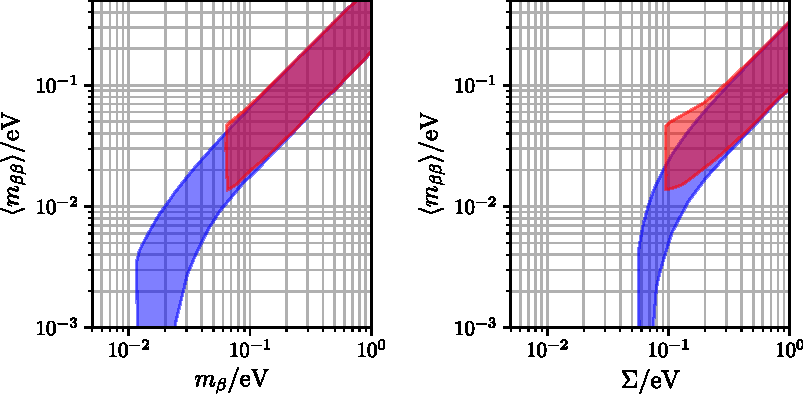
\includegraphics[width=0.9\linewidth]{plots/theory/nu-mass-observables.pdf}
  \caption{%
    The effective mass \mbb\ versus the kinematic neutrino mass observable
    $m_\beta$, and the cosmological observable $\Sigma$. The neutrino
    oscillation parameters are varied within their $3\sigma$ ranges. The blue
    (red) area is for the normal (inverted) mass ordering. Taken
    from~\cite{Dolinski2019}.
  }\label{fig:nbb:mass-obs}
\end{figure}

In this case, no neutrinos are emitted during
the process and the experimental signature is therefore a Dirac-delta function at \qbb\
in the summed energy spectrum (\cref{fig:nbb:spectra}).  A nucleus which can
decay through a \nnbb\ process could also decay through a \onbb\ process, albeit
with a different lifetime ($\gtrsim 10^{25}$~yr). Also the other double-beta
decay modes mentioned in \cref{sec:nbb:2nbb} have their neutrinoless analog.

Considerable experimental efforts are being dedicated to the detection of
\onbb, as such experiments represent the only practical way of establishing
the nature of neutrino mass and therefore of shedding light on the mechanism of
the tiny (but non-zero) neutrino mass generation established by neutrino
oscillation experiments.

\section{Neutrinoless double-beta decay with Majoron emission}

As mentioned in \cref{sec:nbb:0nbb}, the Majorana nature of the neutrino leads
to the violation of the baryon-lepton number $U(1)_{B-L}$ by two units.
Assuming the symmetry is global and its breaking occurs spontaneously, a
massless Nambu-Goldstone boson, called the Majoron (denoted~$\chi$), must exist
in the theory~\cite{Chikashige1981, Schechter1982, Gelmini1981, Georgi1981,
Mohpatra2004}.  Models with massless Majorons have been studied extensively in
the `80, where the Majoron is either a singlet~\cite{Chikashige1981} or part of
a doublet or a triplet~\cite{Gelmini1981, Georgi1981}. However, the last two
possibilities can be ruled out by measurements of the $Z_0$ invisible width at
particle colliders, because of the coupling of the $Z_0$ to the
Majoron~\cite{Berezhiani1992}. All the mentioned models predict neutrinoless
double-beta decay with Majoron emission:
\[
  0\nu\beta\beta\chi:\quad
    \mathcal{N}(A,Z) \longrightarrow \mathcal{N}(A,Z+2) + 2e^- + \chi
\]
the Feynman diagram is shown in \cref{fig:nbb:majfeydiag}, left. Since the
coupling strength of the singlet `seesaw' Majoron is proportional to $m_\nu /
\Lambda$, where $\Lambda$ is the lepton number breaking energy scale (i.e.~the
heavy right-handed neutrino mass in the seesaw mechanism), obtaining observable
decay rates for \onbbx\ and preserving existing bounds on neutrino masses would
require a severe fine-tuning in the theory~\cite{Burgess1993, Burgess1994}.

Another possibility for neutrinoless double-beta decay with Majoron emission
arises in supersymmetric models with R-parity violation~\cite{Masiero1990,
Mohpatra2004}, in which the emission of two Majorons is also
allowed~\cite{Mohpatra1988}:
\[
  0\nu\beta\beta\chi\chi:\quad
    \mathcal{N}(A,Z) \longrightarrow \mathcal{N}(A,Z+2) + 2e^- + 2\chi
\]
See \cref{fig:nbb:majfeydiag} (right) for the Feynman diagram of the process.

To overcome the fine-tuning problem, many alternative models have been
developed starting from the `90. In this class of models, the term `Majoron'
refers more generically to a light or massless boson, not necessarily a
Goldstone scalar boson, that couples to the neutrino. There are models which
foresee Majorons carrying leptonic charge, thus assuring lepton number
conservation and forbidding \onbb. For the case of Majorons with $L = −2$,
\onbbx\ is expected~\cite{Burgess1993}, while $L = −1$ for the Majoron leads to
\onbbxx~\cite{Burgess1994}. Other models make use of a vector Majoron which
becomes the longitudinal component of a massive gauge boson emitted in
double-beta decay~\cite{Carone1993}, which we will also refer to as `Majoron'
in the latter. A decay process that involves the emission of two Majorons is
also possible~\cite{Bamert1995}.  In~\cite{Mohpatra2000}, the model of a `bulk'
Majoron was proposed within models featuring extra dimensionalities
(`brane-bulk' scenario for elementary-particle physics).

For the sake of completeness, it has to be mentioned that in recent years
models with massive Majorons (\cite{Blum2018} and references therein) have
progressively gained popularity, being this kind of Majoron an appealing dark
matter particle candidate. This hypothesis remains however largely untested
from the experimental point of view, because of the additional level of
complexity added to the double-beta event analysis.

\begin{figure}
  \centering%
  \makebox[\textwidth]{%
    \includegraphics[width=0.5\textwidth]{plots/theory/0nbbxfey.pdf}%
    \includegraphics[width=0.5\textwidth]{plots/theory/0nbbxxfey.pdf}%
  }
  \caption{%
    Feynman graphs for neutrinoless double-beta decay with single (right) and
    double (left) Majoron emission. \fillme{not sure about the two-Majoron diagram.}
  }\label{fig:nbb:majfeydiag}
\end{figure}

\marginnote{decay \\ rate}
Independently of the model, the decay rate for double-beta decay with Majoron
emission can be written as:
\begin{align*}
  \Gamma^{0\nu\chi}  &= g_\alpha^2 \cdot G_\alpha^{0\nu\chi}(Q_{\beta\beta}, Z)
    \cdot |M_\alpha^{0\nu\chi}|^2 \\
  \Gamma^{0\nu\chi\chi} &= g_\alpha^4 \cdot G_\alpha^{0\nu\chi\chi}(Q_{\beta\beta}, Z)
    \cdot |M_\alpha^{0\nu\chi\chi}|^2 \;,
\end{align*}
where $g_\alpha$ is the effective coupling constant and $\alpha$ denotes the
model considered. The phase space factors can be parametrized as a
function of \qbb, the sum kinetic energy of the two electrons emitted in
the decay $K$ and the spectral index $n$:
\[
  G_\alpha^{0\nu\chi(\chi)}(Q_{\beta\beta}, Z) \sim (Q_{\beta\beta} - K)^n \;.
\]
$n = 5$ corresponds to the standard \nnbb\ (cfr.~\cref{eq:nbb:stdmodel})
whereas \onbbx\ can have $n = 1, 2, 3$ and \onbbxx\ can have $n = 3, 7$,
depending on the model. As a consequence, the energy spectrum of the two
emitted electrons allows to distinguish the different models. The energy
spectra for all modes of the Majoron emitting double beta decay are shown in
\cref{fig:nbb:majorons-spectra}.

\begin{figure}
  \centering
  \includegraphics{plots/theory/majorons-spectra.pdf}
  \caption{%
    Two-electron energy spectra from different models (labeled by the spectral
    index $n$, see text) of double-beta decay of \gesix, including the standard
    \nnbb, the Lorentz-violating mode \nnbblv\ and the Majoron emitting
    modes.  Analytic formulas, obtained with the Primakoff-Rosen approximation,
    for the Fermi function are taken from~\cite{Tretyak1995, Tretyak2002}.
  }\label{fig:nbb:majorons-spectra}
\end{figure}

\section{Lorentz-violating two-neutrino double-beta decay}

Since the Standard Model of Particle Physics is known to provide a successful
description of most physics at low energies, compared to the Planck scale
$m_p\sim10^{19}$~GeV, any signal of new physics must appear at low energies in
the form of an effective quantum field theory containing the Standard Model.
The general effective quantum field theory constructed from the latter and
allowing for arbitrary coordinate-independent Lorentz violation is called the
Standard Model Extension~\cite{Colladay1997, Colladay1998}. As an effective
field theory it provides a link to the Planck scale through operators of
non-renormalizable dimension. The Lagrangian of the Standard Model Extension
consists of the usual Standard Model Lagrangian supplemented by all possible
terms that can be constructed with the existing fields and that introduce
violations of Lorentz symmetry. The additional terms have the form of
Lorentz-violating operators coupled to vector coefficients, and they could
arise in a variety of ways.

All quantum field operators for Lorentz violation involved in the propagation
of neutrinos have been classified and enumerated~\cite{Kostelecky2012}. Most of
these can be studied using neutrino oscillations, which compare the way
different neutrinos propagate and provide interferometric sensitivity to energy
differences between them. Some effects cannot be detected by neutrino
oscillations because they are produced by ‘oscillation-free’ operators that
change all neutrino energies equally. Most of these can instead be studied by
comparing neutrino propagation to other species, such as time-of-flight
experiments matching the group velocity of neutrinos with the photons' one.
However, four oscillation-free operators leave unaffected the neutrino group
velocity and so cannot be detected in this way. Instead, they must be accessed
through physical processes that involve neutrino phase-space properties, such
as particle decays. These operators are rare examples of \textit{countershaded}
Lorentz violations~\cite{Kostelecky2009}: Relativity-violating effects that could
be enormous compared to ones suppressed by the ratio $m_W/m_P$ and that
nonetheless could have escaped detection to date. These could provide an
interesting path for building models with viable Lorentz violation obviating
the typical requirement of a heavy suppression factor.

The four countershaded neutrino operators are of renormalizable mass dimension
$d = 3$, are odd under \cpt, and are controlled by coefficients conventionally
denoted with $(a^{(3)}_\text{of})_{jm}$, where $j$, $m$ are angular-momentum
quantum numbers with $j = 0,1$. Conservation of energy and momentum is assured
by taking these four coefficients to be constant as usual for couplings beyond
the Standard Model, so all physics other than Lorentz and \cpt\ violation is
conventional. Dimensional arguments suggest these coefficients are likely to
dominate at accessible energies and can be measured sensitively in low-energy
processes.

The anti-neutrino phase space element $\text{d}^3q$ is modified by the presence
of these new operators:
\[
  \omega^2\text{d}\omega\text{d}\Omega \;\longmapsto\;
    f(\omega)\text{d}\omega\text{d}\Omega\;,
\]
where the anti-neutrino function
\[
  f(\omega)\simeq\omega^2-\frac{1}{2}m_\nu^2-2\omega\delta\omega
\]
encodes the Lorentz-violating modifications
\[
  \delta\omega = -\sum_{jm} e^{im\omega_\oplus T_\oplus}
    \mathcal{N}_{jm}(a_\text{of}^{(3)})_{jm}
\]
arising from the modified anti-neutrino dispersion
relation~\cite{Kostelecky2012} $\omega = |\mathbf{q}| + m_\nu^2 / |\mathbf{q}|
+ \delta\omega$. The sidereal time $T_\oplus$ controls the harmonic variation
of the anti-neutrino function in the laboratory produced by the Earth sidereal
rotation at frequency $\omega_\oplus \simeq 2\pi/(23\text{h}~56\text{min})$.
The factors $\mathcal{N}_{jm}$ contain information about the direction of
propagation of the anti-neutrinos, expressed relative to the canonical
sun-centered frame of reference~\cite{Bluhm2003, Kostelecky2002}.

\marginnote{decay \\ rate}
Following the same procedure as in the conventional two-neutrino double-beta
decay, we integrate over all orientation, which implies that only isotropic
effects are observable and hence that the residual spectrum depends only on
$\aof\equiv{(a_\text{of}^{(3)})}_{00}/\sqrt{4\pi}$. After a suitable change of
integration variables and defining the sum of kinetic energies $K=T_1+T_2$ for
the two electrons, we obtain the electron sum spectrum
\begin{equation}\label{eq:nbb:totwidth}
  \begin{split}
    \frac{\text{d}\Gamma}{\text{d}K} = &
      \Lambda \cdot (K^5 + 10K^4 + 40K^3 + 60K^2 + 30K) \\
      & \times[(Q_{\beta\beta} - K)^5 + 10\aof(Q_{\beta\beta} - K)^4] \;. \\
  \end{split}
\end{equation}
The total decay rate can be therefore expressed as an addition of two separate
rates through a perturbation:
\[
  \Gamma = \Gamma_0 + \delta\Gamma \;,
\]
where the first term is (\ref{eq:nbb:stdmodel}) and the second one contains all the
new Lorentz-violating information. The two differential decay rates are
depicted in \cref{fig:nbb:majorons-spectra}.

\marginnote{experimental \\ limits}
Conservative constraints on the $(\mathring{a}^{(3)}_\text{of})_{00}$
coefficient have been placed using published results from the Troitsk and Mainz
experiments studying the endpoint of the tritium beta decay energy spectrum
\cite{Diaz:2013saa}. An outside analysis of data from the two experiments gives
$|(\mathring{a}^{(3)}_\text{of})_{00}|<2\cdot10^{-8}$~GeV for both of them.
Constraints on the values of $\aof$ have also been extracted from studies of
threshold effects in pion and kaon decays \cite{SMEneutrinos}, yielding
$\aof<1.9\cdot10^{-7}$~GeV as the best upper limit.

A constraint from double-beta decay studies has been posed by the EXO-200
collaboration in ref.~\cite{exo200}. A profile Likelihood scan over the number
of Lorentz-violating double beta decay integral counts added to the standard
\nnbb\ spectrum is used to obtain a limit at the 90\% C.L, which is
$\aof<7.6\cdot10^{-6}$~GeV. This is the first search for this parameter that
fully accounts for experimental backgrounds and detector-related systematic
uncertainties.
